\documentclass[preprint,12pt,authoryear]{elsarticle}
\usepackage[utf8]{inputenc}
\usepackage[T1]{fontenc}
\usepackage{amsmath,amssymb}
\usepackage{booktabs}
\usepackage{graphicx}
\usepackage{url}
\usepackage[hidelinks]{hyperref}
\usepackage{lineno}
\usepackage{adjustbox}
\biboptions{authoryear}

\newcommand{\DeltaSteels}{-0.3202}
\newcommand{\RelSteels}{-0.39}
\newcommand{\PNBSteels}{0.896}
\newcommand{\PBootSteels}{0.720}
\newcommand{\PHolmSteels}{1.000}
\newcommand{\FoldsSteels}{3}
\newcommand{\SteelsStack}{83.12}
\newcommand{\SteelsStackStd}{10.89}
\newcommand{\SteelsStackLocal}{82.80}
\newcommand{\SteelsStackLocalStd}{11.65}
\newcommand{\SteelsStackFm}{82.02}
\newcommand{\SteelsStackFmStd}{9.12}
\newcommand{\SteelsBestSingle}{83.41}
\newcommand{\SteelsBestSingleStd}{10.86}
\newcommand{\SteelsMeanEnsemble}{102.46}
\newcommand{\SteelsMeanEnsembleStd}{20.11}
\newcommand{\SteelsSingleLocal}{82.69}
\newcommand{\SteelsSingleLocalStd}{11.60}
\newcommand{\SteelsStackLocalVsBestSingleRel}{-0.74}
\newcommand{\SteelsStackLocalVsBestSingleP}{0.538}
\newcommand{\SteelsStackLocalVsBestSingleFolds}{3}
\newcommand{\SteelsStackVsBestSingleRel}{-0.35}
\newcommand{\SteelsStackVsBestSingleP}{0.660}
\newcommand{\SteelsStackVsBestSingleFolds}{2}
\newcommand{\SteelsSingleLocalVsBestSingleRel}{-0.86}
\newcommand{\SteelsSingleLocalVsBestSingleP}{0.425}
\newcommand{\SteelsSingleLocalVsBestSingleFolds}{3}
\newcommand{\SteelsStackLocalVsMeanEnsembleRel}{-19.19}
\newcommand{\SteelsStackLocalVsMeanEnsembleP}{$<$0.001}
\newcommand{\SteelsStackLocalVsMeanEnsembleFolds}{5}
\newcommand{\SteelsStackFmVsStackRel}{-1.32}
\newcommand{\SteelsStackFmVsStackP}{0.519}
\newcommand{\SteelsStackFmVsStackFolds}{2}
\newcommand{\SteelsStackFmVsStackLocalRel}{-0.94}
\newcommand{\SteelsStackFmVsStackLocalP}{0.583}
\newcommand{\SteelsStackFmVsStackLocalFolds}{3}
\newcommand{\SteelsStackLocalMagpieVsStackRel}{+0.50}
\newcommand{\SteelsStackLocalMagpieVsStackP}{0.036}
\newcommand{\SteelsStackLocalMagpieVsStackFolds}{0}
\newcommand{\SteelsStackLocalFracVsStackRel}{-0.39}
\newcommand{\SteelsStackLocalFracVsStackP}{0.721}
\newcommand{\SteelsStackLocalFracVsStackFolds}{3}
\newcommand{\SteelsNaiveOn}{5}
\newcommand{\SteelsFmOn}{5}
\newcommand{\SteelsPermNaiveOn}{5}
\newcommand{\SteelsPermFmOn}{5}
\newcommand{\SteelsFoldZeroStack}{91.07}
\newcommand{\SteelsFoldZeroLocal}{96.23}
\newcommand{\SteelsFoldZeroFm}{95.73}
\newcommand{\SteelsFoldZeroBest}{91.07}
\newcommand{\DeltaGap}{-0.00232}
\newcommand{\RelGap}{-0.71}
\newcommand{\PNBGap}{0.011}
\newcommand{\PBootGap}{0.001}
\newcommand{\PHolmGap}{0.005}
\newcommand{\FoldsGap}{5}
\newcommand{\GapStack}{0.3264}
\newcommand{\GapStackStd}{0.0139}
\newcommand{\GapStackLocal}{0.3240}
\newcommand{\GapStackLocalStd}{0.0140}
\newcommand{\GapStackFm}{0.3276}
\newcommand{\GapStackFmStd}{0.0149}
\newcommand{\GapBestSingle}{0.3259}
\newcommand{\GapBestSingleStd}{0.0130}
\newcommand{\GapMeanEnsemble}{0.4007}
\newcommand{\GapMeanEnsembleStd}{0.0242}
\newcommand{\GapSingleLocal}{0.3239}
\newcommand{\GapSingleLocalStd}{0.0133}
\newcommand{\GapStackLocalVsBestSingleRel}{-0.58}
\newcommand{\GapStackLocalVsBestSingleP}{0.071}
\newcommand{\GapStackLocalVsBestSingleFolds}{4}
\newcommand{\GapStackVsBestSingleRel}{+0.13}
\newcommand{\GapStackVsBestSingleP}{0.566}
\newcommand{\GapStackVsBestSingleFolds}{3}
\newcommand{\GapSingleLocalVsBestSingleRel}{-0.63}
\newcommand{\GapSingleLocalVsBestSingleP}{0.002}
\newcommand{\GapSingleLocalVsBestSingleFolds}{5}
\newcommand{\GapStackLocalVsMeanEnsembleRel}{-19.14}
\newcommand{\GapStackLocalVsMeanEnsembleP}{$<$0.001}
\newcommand{\GapStackLocalVsMeanEnsembleFolds}{5}
\newcommand{\GapStackFmVsStackRel}{+0.38}
\newcommand{\GapStackFmVsStackP}{0.390}
\newcommand{\GapStackFmVsStackFolds}{2}
\newcommand{\GapStackFmVsStackLocalRel}{+1.10}
\newcommand{\GapStackFmVsStackLocalP}{0.005}
\newcommand{\GapStackFmVsStackLocalFolds}{0}
\newcommand{\GapStackLocalMagpieVsStackRel}{-0.86}
\newcommand{\GapStackLocalMagpieVsStackP}{$<$0.001}
\newcommand{\GapStackLocalMagpieVsStackFolds}{5}
\newcommand{\GapStackLocalFracVsStackRel}{-0.88}
\newcommand{\GapStackLocalFracVsStackP}{0.001}
\newcommand{\GapStackLocalFracVsStackFolds}{5}
\newcommand{\GapNaiveOn}{5}
\newcommand{\GapFmOn}{5}
\newcommand{\GapPermNaiveOn}{5}
\newcommand{\GapPermFmOn}{5}
\newcommand{\GapFoldZeroStack}{0.3109}
\newcommand{\GapFoldZeroLocal}{0.3079}
\newcommand{\GapFoldZeroFm}{0.3107}
\newcommand{\GapFoldZeroBest}{0.3114}
\newcommand{\DeltaMetal}{-0.00000}
\newcommand{\RelMetal}{-0.00}
\newcommand{\PNBMetal}{0.541}
\newcommand{\PBootMetal}{0.899}
\newcommand{\PHolmMetal}{1.000}
\newcommand{\FoldsMetal}{0}
\newcommand{\MetalStack}{0.9825}
\newcommand{\MetalStackStd}{0.0017}
\newcommand{\MetalStackBA}{0.9374}
\newcommand{\MetalStackLocal}{0.9825}
\newcommand{\MetalStackLocalStd}{0.0018}
\newcommand{\MetalStackLocalBA}{0.9370}
\newcommand{\MetalStackFm}{0.9826}
\newcommand{\MetalStackFmStd}{0.0017}
\newcommand{\MetalStackFmBA}{0.9366}
\newcommand{\MetalBestSingle}{0.9819}
\newcommand{\MetalBestSingleStd}{0.0015}
\newcommand{\MetalBestSingleBA}{0.9378}
\newcommand{\MetalMeanEnsemble}{0.9811}
\newcommand{\MetalMeanEnsembleStd}{0.0027}
\newcommand{\MetalSingleLocal}{0.9819}
\newcommand{\MetalSingleLocalStd}{0.0015}
\newcommand{\MetalSingleLocalBA}{0.9378}
\newcommand{\MetalStackLocalVsBestSingleRel}{+0.06}
\newcommand{\MetalStackLocalVsBestSingleP}{0.301}
\newcommand{\MetalStackLocalVsBestSingleFolds}{4}
\newcommand{\MetalStackVsBestSingleRel}{+0.06}
\newcommand{\MetalStackVsBestSingleP}{0.275}
\newcommand{\MetalStackVsBestSingleFolds}{4}
\newcommand{\MetalSingleLocalVsBestSingleRel}{+0.00}
\newcommand{\MetalSingleLocalVsBestSingleP}{0.714}
\newcommand{\MetalSingleLocalVsBestSingleFolds}{2}
\newcommand{\MetalStackLocalVsMeanEnsembleRel}{+0.14}
\newcommand{\MetalStackLocalVsMeanEnsembleP}{0.008}
\newcommand{\MetalStackLocalVsMeanEnsembleFolds}{5}
\newcommand{\MetalStackFmVsStackRel}{+0.02}
\newcommand{\MetalStackFmVsStackP}{0.320}
\newcommand{\MetalStackFmVsStackFolds}{3}
\newcommand{\MetalStackFmVsStackLocalRel}{+0.02}
\newcommand{\MetalStackFmVsStackLocalP}{0.277}
\newcommand{\MetalStackFmVsStackLocalFolds}{3}
\newcommand{\MetalStackLocalMagpieVsStackRel}{+0.00}
\newcommand{\MetalStackLocalMagpieVsStackP}{1.000}
\newcommand{\MetalStackLocalMagpieVsStackFolds}{0}
\newcommand{\MetalStackLocalFracVsStackRel}{-0.00}
\newcommand{\MetalStackLocalFracVsStackP}{0.898}
\newcommand{\MetalStackLocalFracVsStackFolds}{0}
\newcommand{\MetalNaiveOn}{1}
\newcommand{\MetalFmOn}{5}
\newcommand{\MetalPermNaiveOn}{5}
\newcommand{\MetalPermFmOn}{5}
\newcommand{\MetalFoldZeroStack}{0.9850}
\newcommand{\MetalFoldZeroLocal}{0.9850}
\newcommand{\MetalFoldZeroFm}{0.9848}
\newcommand{\MetalFoldZeroBest}{0.9838}
\newcommand{\DeltaGlass}{+0.00000}
\newcommand{\RelGlass}{+0.00}
\newcommand{\PNBGlass}{1.000}
\newcommand{\PBootGlass}{1.000}
\newcommand{\PHolmGlass}{1.000}
\newcommand{\FoldsGlass}{0}
\newcommand{\GlassStack}{0.9567}
\newcommand{\GlassStackStd}{0.0091}
\newcommand{\GlassStackBA}{0.8841}
\newcommand{\GlassStackLocal}{0.9567}
\newcommand{\GlassStackLocalStd}{0.0091}
\newcommand{\GlassStackLocalBA}{0.8841}
\newcommand{\GlassStackFm}{0.9559}
\newcommand{\GlassStackFmStd}{0.0094}
\newcommand{\GlassStackFmBA}{0.8835}
\newcommand{\GlassBestSingle}{0.9548}
\newcommand{\GlassBestSingleStd}{0.0097}
\newcommand{\GlassBestSingleBA}{0.8827}
\newcommand{\GlassMeanEnsemble}{0.9458}
\newcommand{\GlassMeanEnsembleStd}{0.0116}
\newcommand{\GlassSingleLocal}{0.9548}
\newcommand{\GlassSingleLocalStd}{0.0097}
\newcommand{\GlassSingleLocalBA}{0.8827}
\newcommand{\GlassStackLocalVsBestSingleRel}{+0.20}
\newcommand{\GlassStackLocalVsBestSingleP}{0.002}
\newcommand{\GlassStackLocalVsBestSingleFolds}{5}
\newcommand{\GlassStackVsBestSingleRel}{+0.20}
\newcommand{\GlassStackVsBestSingleP}{0.002}
\newcommand{\GlassStackVsBestSingleFolds}{5}
\newcommand{\GlassSingleLocalVsBestSingleRel}{+0.00}
\newcommand{\GlassSingleLocalVsBestSingleP}{1.000}
\newcommand{\GlassSingleLocalVsBestSingleFolds}{0}
\newcommand{\GlassStackLocalVsMeanEnsembleRel}{+1.15}
\newcommand{\GlassStackLocalVsMeanEnsembleP}{$<$0.001}
\newcommand{\GlassStackLocalVsMeanEnsembleFolds}{5}
\newcommand{\GlassStackFmVsStackRel}{-0.09}
\newcommand{\GlassStackFmVsStackP}{0.153}
\newcommand{\GlassStackFmVsStackFolds}{1}
\newcommand{\GlassStackFmVsStackLocalRel}{-0.09}
\newcommand{\GlassStackFmVsStackLocalP}{0.149}
\newcommand{\GlassStackFmVsStackLocalFolds}{1}
\newcommand{\GlassStackLocalMagpieVsStackRel}{+0.00}
\newcommand{\GlassStackLocalMagpieVsStackP}{1.000}
\newcommand{\GlassStackLocalMagpieVsStackFolds}{0}
\newcommand{\GlassStackLocalFracVsStackRel}{+0.00}
\newcommand{\GlassStackLocalFracVsStackP}{1.000}
\newcommand{\GlassStackLocalFracVsStackFolds}{0}
\newcommand{\GlassNaiveOn}{0}
\newcommand{\GlassFmOn}{5}
\newcommand{\GlassPermNaiveOn}{5}
\newcommand{\GlassPermFmOn}{5}
\newcommand{\GlassFoldZeroStack}{0.9694}
\newcommand{\GlassFoldZeroLocal}{0.9694}
\newcommand{\GlassFoldZeroFm}{0.9699}
\newcommand{\GlassFoldZeroBest}{0.9690}
\newcommand{\NTasksImproved}{1}
\newcommand{\SteelsRank}{3}
\newcommand{\SteelsNEntries}{12}
\newcommand{\SteelsBoardBest}{TPOT-Mat}
\newcommand{\GapRank}{2}
\newcommand{\GapNEntries}{13}
\newcommand{\GapBoardBest}{Darwin}
\newcommand{\MetalAUCprob}{0.9825}
\newcommand{\MetalRank}{2}
\newcommand{\MetalNEntries}{8}
\newcommand{\MetalBoardBest}{Darwin}
\newcommand{\GlassAUCprob}{0.9567}
\newcommand{\GlassRank}{2}
\newcommand{\GlassNEntries}{8}
\newcommand{\GlassBoardBest}{MODNet (v0.1.12)}
\newcommand{\SteelsWallMin}{1}
\newcommand{\GapWallMin}{8}
\newcommand{\MetalWallMin}{4}
\newcommand{\GlassWallMin}{5}
\newcommand{\TotalCPUhWall}{1.5}
\newcommand{\SteelsScratchMin}{1}
\newcommand{\GapScratchMin}{16}
\newcommand{\MetalScratchMin}{8}
\newcommand{\GlassScratchMin}{44}
\newcommand{\SteelsPairShare}{44}
\newcommand{\GapPairShare}{33}
\newcommand{\MetalPairShare}{37}
\newcommand{\GlassPairShare}{84}
\newcommand{\SteelsLocalQOne}{+6.8}
\newcommand{\SteelsFmQOne}{-0.8}
\newcommand{\SteelsLocalQTwo}{-1.7}
\newcommand{\SteelsFmQTwo}{-2.8}
\newcommand{\SteelsLocalQThree}{-2.1}
\newcommand{\SteelsFmQThree}{+1.5}
\newcommand{\SteelsLocalQFour}{-1.5}
\newcommand{\SteelsFmQFour}{-2.2}
\newcommand{\GapLocalQOne}{+0.9}
\newcommand{\GapFmQOne}{+2.0}
\newcommand{\GapLocalQTwo}{-1.0}
\newcommand{\GapFmQTwo}{+0.5}
\newcommand{\GapLocalQThree}{-1.1}
\newcommand{\GapFmQThree}{+0.2}
\newcommand{\GapLocalQFour}{-0.9}
\newcommand{\GapFmQFour}{-0.3}
\newcommand{\MetalLocalQOne}{-0.1}
\newcommand{\MetalFmQOne}{+1.1}
\newcommand{\MetalLocalQTwo}{+0.0}
\newcommand{\MetalFmQTwo}{-1.0}
\newcommand{\MetalLocalQThree}{-0.2}
\newcommand{\MetalFmQThree}{+0.7}
\newcommand{\MetalLocalQFour}{-0.0}
\newcommand{\MetalFmQFour}{-0.6}
\newcommand{\GlassLocalQOne}{+0.0}
\newcommand{\GlassFmQOne}{+3.0}
\newcommand{\GlassLocalQTwo}{+0.0}
\newcommand{\GlassFmQTwo}{+0.8}
\newcommand{\GlassLocalQThree}{+0.0}
\newcommand{\GlassFmQThree}{-0.9}
\newcommand{\GlassLocalQFour}{+0.0}
\newcommand{\GlassFmQFour}{+0.8}


\journal{Computational Materials Science}

\begin{document}

\begin{frontmatter}

\title{A pre-registered test of cross-fitted stacking with a novelty-damped local residual correction on the Matbench composition tasks}

\author{Bhaskar Gurram}
\ead{gurrambhaskar.ai@gmail.com}
\affiliation{organization={Independent Researcher}}

\begin{abstract}
We evaluate cross-fitted stacking of composition-based experts on the four composition tasks of Matbench v0.1 (steels, expt\_gap, expt\_is\_metal, glass).
The protocol is the same for both runs:
\begin{itemize}
\item only the official folds are used;
\item every model, hyperparameter and design choice is made by cross-validation inside each training fold;
\item the analysis plan was written, and the code frozen by SHA-256 hash, before the test folds were scored.
\end{itemize}

\textbf{First pre-registered run.} It tested whether a novelty-damped local out-of-fold residual correction, confirmed in earlier chemistry work, transfers to materials. It transferred only weakly: a 0.7\% MAE gain on the experimental band gap (5/5 folds, Holm-adjusted $p=\PHolmGap$), and no effect elsewhere.

\textbf{Second pre-registered run.} Written after the first results were seen, and disclosed as such, it strengthened the pipeline with:
\begin{itemize}
\item further label-free descriptors;
\item a transfer-learning block of DFT (PBE) gaps and formation energies from offline Materials Project data;
\item a hurdle treatment of the zero-inflated band gap;
\item Optuna-tuned gradient boosting;
\item a nested-CV gate for the local correction, which then kept the correction in none of the 20 folds.
\end{itemize}

Against the leaderboard leaders, paired over the same test compositions with their public predictions:
\begin{itemize}
\item \textbf{expt\_gap:} our MAE is \AtwoFinalGap{}~eV against \AtwoLeaderGap{}~eV for the best entry (\AtwoPHolmExprGap).
\item \textbf{expt\_is\_metal:} on par (balanced accuracy \AtwoFinalMetal{} vs.\ \AtwoLeaderMetal).
\item \textbf{steels:} on par (MAE \AtwoFinalSteels{} vs.\ \AtwoLeaderSteels~MPa).
\item \textbf{glass:} behind (\AtwoFinalGlass{} vs.\ \AtwoLeaderGlass).
\end{itemize}
We also show that the leaders of the classification tasks are scored by balanced accuracy, not probability ROC-AUC.
Everything ran on one 24-core CPU workstation.
\end{abstract}


\begin{keyword}
materials informatics \sep composition-based property prediction \sep Matbench \sep stacking \sep residual correction \sep nested cross-validation \sep pre-registration
\end{keyword}

\end{frontmatter}

\linenumbers

\section{Introduction}
\label{sec:intro}

Composition-only property models remain the workhorse of materials screening whenever the crystal structure is unknown, and the Matbench v0.1 suite \citep{dunn2020matbench} has become the common yardstick for them.
Four of its tasks are composition-only and comparatively small: the yield strength of steels (312 alloys), the experimental band gap (4,604 compounds), the experimental metal/non-metal label (4,921) and glass-forming ability (5,680).
On these tasks the leaderboard \citep{matbenchboard} is led by quite different model families: automated machine-learning pipelines on steels, feature-selected neural networks (MODNet, \citealp{debreuck2021modnet}) on glass, and the Darwin entry on the two experimental band-gap tasks.
The composition models we are aware of either fit one global predictor or combine predictors with weights that are the same for every composition (as automated-ML ensembles and stacked models do) \citep{debreuck2021modnet,wang2021crabnet,goodall2020roost,gouvea2025mattervial,zou2025ecsg}.

Errors of such models are rarely uniform over composition space.
Chemical families share systematic biases, and a residual that is large for one alloy is often large for its neighbours.
In geostatistics this observation underlies regression kriging, where a trend model is followed by interpolation of its residuals \citep{hengl2007rk}; in quantum chemistry, $\Delta$-learning corrects a cheap baseline with a learned residual \citep{ramakrishnan2015delta}.
In earlier work on chemical property prediction (SIG-Net, \citealp{gurram2026signet}) we combined a cross-fitted stack of diverse experts \citep{wolpert1992stacked,breiman1996stacked,vanderlaan2007super} with a \emph{novelty-damped local out-of-fold (OOF) residual correction}: each prediction is shifted by a kernel-weighted average of the OOF residuals of its nearest training neighbours, and the shift is damped where the query is far from all of them.
That correction was confirmed in a pre-registered replication.

Here we ask whether the same construction transfers to composition-based materials property prediction, under the strictest protocol we could devise on a public benchmark:
(i) only the official Matbench folds are used;
(ii) every choice (expert hyperparameters, stacking weights, correction strength, neighbourhood size, bandwidth, damping and kernel space) is made by cross-validation inside each training fold;
(iii) the analysis plan, endpoints and tests were written and the code was frozen by cryptographic hash before any official test fold was predicted; and
(iv) every task, fold and arm is reported.
We also test a variant suggested by a structured ideation-and-review process (Section~\ref{sec:fm}): a \emph{fold-matched} correction that removes a double-counting term which arises because the deployed stack has already been trained on the neighbours whose residuals it borrows.

\section{Related work}
\label{sec:related}

\paragraph{Composition models on Matbench}
Magpie descriptors with random forests \citep{ward2016magpie} and the Automatminer reference \citep{dunn2020matbench} established the baselines; MODNet \citep{debreuck2021modnet,debreuck2021bias} added relevance-redundancy feature selection and joint learning for small data; CrabNet \citep{wang2021crabnet} and Roost \citep{goodall2020roost} learn representations directly from stoichiometry; MatterVial fuses latent, symbolic and descriptor features into a MODNet model \citep{gouvea2025mattervial}; and tabular foundation models such as TabPFN \citep{hollmann2025tabpfn} are now competitive on small tabular sets.
None of these adapts its prediction to the residual structure of nearby training compositions.

\paragraph{Ensembles and stacking for materials}
Stacked ensembles have been used for experimental band gaps with DFT-trained first-layer models \citep{kauwe2020bandgap}, for thermodynamic stability from electron-configuration and other composition models \citep{zou2025ecsg}, and for alloy mechanical properties on single datasets with random splits (e.g.\ \citealp{zhao2025hea}).
A mixture of experts over pretrained extractors addresses data scarcity \citep{chang2022moe}, and an ``ensemble of experts'' built from networks pre-trained on related polymer properties was recently proposed in this journal \citep{miccio2025ee}; the latter is transfer learning from SMILES and contains no stacking or residual stage.

\paragraph{Residual correction}
Regression kriging \citep{hengl2007rk} and $\Delta$-learning \citep{ramakrishnan2015delta} are the closest classical analogues of a local residual correction.
A recent preprint corrects a convex neural stack by global kernel-ridge regression of its residuals in operator learning \citep{shmalo2026kernel}.
None of these uses OOF residuals with novelty damping in composition space, or evaluates on Matbench folds; the method itself, however, is not new in its components, and our contribution is the pre-registered transfer test, the fold-matched variant and the analysis of where the correction helps or hurts.
A structured prior-art check (details in the Supplementary Material) rated the overlap as medium: every component has ancestors, but we found no work that combines them on these tasks.

\section{Methods}
\label{sec:methods}

\subsection{Data, splits and features}
We use the four composition tasks of Matbench v0.1 through the \texttt{matbench} package (\texttt{MatbenchBenchmark}), with the official five folds; nothing is re-split.
Each composition is described by label-free features computed with \texttt{matminer} \citep{ward2018matminer} and \texttt{pymatgen} \citep{ong2013pymatgen}: 132 Magpie element-property statistics \citep{ward2016magpie}, 103 element fractions, and 21 further descriptors (stoichiometric norms, valence-orbital fractions \citep{meredig2014}, ionic character and charge-balance flags, band centre and atomic-orbital HOMO/LUMO estimates).
A handful of compositions (0, 14, 14 and 21 rows in the four tasks) make one of the extra featurisers fail; these values are imputed with the feature's dataset-wide median, which uses no labels.

\subsection{Experts and cross-fitting}
Inside an official training fold $T_k$ the training rows are split into $J=5$ inner folds $P_1,\dots,P_J$ (seed 0; stratified for classification).
Every expert $e$ is fitted $J$ times on $T_k\setminus P_m$ to produce OOF predictions $\hat f_e^{(-m(i))}(x_i)$, and once on all of $T_k$ to predict the test rows.
The expert pool is deliberately heterogeneous and CPU-feasible: LightGBM \citep{ke2017lightgbm} on all features (for expt\_gap also an L1-objective copy), random forests \citep{breiman2001rf}, extremely randomised trees \citep{geurts2006et}, kernel ridge regression on element fractions and on standardised Magpie features (RBF kernel, regularisation and width chosen by an internal three-fold grid search), RBF support-vector classifiers on the same two spaces for the classification tasks, and a two-layer perceptron \citep{pedregosa2011sklearn}.
Regression predictions are clipped to the training-target range.

\subsection{Simplex stack}
The global stack is $s(x)=\sum_e w_e \hat f_e(x)$ with $w_e\ge 0$ and $\sum_e w_e=1$, fitted on the OOF predictions.
For regression the weights minimise the mean absolute error (a linear programme, matching the Matbench metric); for classification they minimise the Brier score.
To obtain OOF \emph{stack} predictions $s^{\mathrm{oof}}(x_i)$ for the training rows, the weights used for inner fold $m$ are fitted without the rows of $P_m$.

\subsection{Novelty-damped local OOF residual correction}
\label{sec:naive}
With OOF residuals $r_j = y_j - s^{\mathrm{oof}}(x_j)$, the corrected prediction for a query $q$ is
\begin{equation}
\hat y(q) = s(q) + \alpha\,\frac{\sum_{j\in\mathcal N_k(q)} w_{qj}\,r_j}{\sum_{j\in\mathcal N_k(q)} w_{qj} + \kappa},
\qquad w_{qj}=\exp\!\big(-(d(q,j)/h)^2\big),
\label{eq:naive}
\end{equation}
where $\mathcal N_k(q)$ are the $k$ nearest training compositions under a composition distance $d$ (Euclidean on standardised Magpie vectors, or L1 on element fractions).
The pseudo-count $\kappa$ provides the novelty damping: when all neighbours are far, $\sum w$ is small and the correction vanishes.
For classification the shift is applied on the logit scale with probability residuals.
The tuple $(d,k,h,\kappa,\alpha)$ is selected on the training rows only, by scoring the corrected OOF predictions (leave-self-out neighbour sets) with the task metric over a fixed grid: $k\in\{5,10,20,40\}$, $h$ a multiple $\{0.5,1,2,4,8,16\}$ of the median nearest-neighbour distance, $\kappa\in\{0,0.1,0.5,2\}$, and $\alpha\in\{0.25,0.5,0.75,1\}$ (regression) or $\{0.1,0.25,0.5,1,2,4\}$ (classification).
The uncorrected stack ($\alpha=0$) is always a candidate and wins ties, so the procedure may decline to correct.

\subsection{Fold-matched correction}
\label{sec:fm}
The deployed stack $s=F^{\mathrm{full}}$ was trained on the very neighbours $j$ whose OOF residuals Eq.~\eqref{eq:naive} borrows.
Writing $F^{(-m)}$ for the stack whose experts excluded inner fold $P_m$, the naive transfer decomposes as $r_j = [r_j + F^{(-m(j))}(q) - F^{\mathrm{full}}(q)] + [F^{\mathrm{full}}(q)-F^{(-m(j))}(q)]$.
The second bracket, the \emph{absorption term}, measures how far the refit has already moved toward the neighbour, and the naive correction counts it a second time; for interpolating experts and near-duplicate neighbours it can be as large as $r_j$ itself.
The fold-matched variant transfers only the first bracket, $T_{qj}=r_j + F^{(-m(j))}(q) - F^{\mathrm{full}}(q)$, in place of $r_j$ in Eq.~\eqref{eq:naive}.
Its selection uses deployment-matched training instances: for a training row $i\in P_m$ and a neighbour $j\in P_{m'}$ ($m'\neq m$) the transfer is computed from the pair-excluded refit $F^{(-m,-m')}$, which saw neither $i$ nor $j$; neighbours in the same inner fold use $r_j$ directly.
This requires $J(J-1)/2=10$ extra fits per expert and fold, with the stack weights held fixed.
The variant was proposed by a structured ideation pipeline (ResearchStudio IdeaSpark), whose coherence check verified the algebraic decomposition on synthetic instances; we pre-registered it as a secondary arm, not as the primary method.
Relative to that proposal we simplified the damping map to the same $(\alpha,\kappa)$ family as Eq.~\eqref{eq:naive}, used the same two distances instead of the element mover's distance, and did not add TabPFN or MODNet experts, for reasons of CPU cost.

\subsection{Hard labels for classification}
Most classification entries on the Matbench leaderboard report a ``ROC-AUC'' equal to their balanced accuracy, which is what \texttt{matbench} computes when hard labels rather than probabilities are recorded.
For a like-for-like comparison we therefore also report balanced accuracy at a threshold chosen inside each training fold (maximising balanced accuracy on the arm's training OOF predictions), alongside the probability ROC-AUC.

\subsection{Protocol, pre-registration and statistics}
\label{sec:protocol}
All model and hyperparameter selection was done by cross-validation within each official training fold.
Concretely, the candidate design configurations (with or without the 21 extra descriptors; L2 or L1 stacking loss; with or without an L1-objective LightGBM expert) were first explored by inner cross-validation on the training rows of fold~0 only.
Then, inside every official training fold $T_k$, all candidates were cross-fitted and the one with the best cross-fitted OOF score of the uncorrected global stack was kept; because this criterion uses the uncorrected stack, it favours neither correction arm.
The correction hyperparameters were then selected inside $T_k$ as described above.
The analysis plan, including an amendment that introduced this per-fold selection and was written before any official test fold was scored, and the SHA-256 hashes of all code were committed before the final run; both are provided in the repository and Supplementary Material.
(An earlier run under the original plan, in which the design was fixed on fold~0's training rows, was stopped and never scored.)

The primary endpoint, per task, is $\Delta$ = mean over the five official folds of the metric of the corrected stack minus that of the uncorrected stack (MAE for regression, probability ROC-AUC for classification).
Its test is a paired bootstrap that resamples test points within folds ($B=10{,}000$), with Holm correction across the four tasks; a task counts as improved only if $\Delta$ favours the correction and the Holm-adjusted $p<0.05$.
Because five folds give little power, we also report per-fold differences, the number of folds improved, and the Nadeau--Bengio corrected resampled $t$-test \citep{nadeau2003inference}.
Secondary comparisons (fold-matched versus stack and versus naive, stack versus the best single expert selected by inner CV, kernel-space ablations, correction without stacking) and analyses (errors stratified by distance to the nearest training composition, calibration, selected configurations, and a label-permutation control) were also pre-specified.

\section{Results I: the transferred local correction (Amendment 1)}
\label{sec:results}

\subsection{All arms on the official folds}
Table~\ref{tab:arms} lists every arm on every task (mean $\pm$ standard deviation over the five official folds), and Table~\ref{tab:tests} the pre-registered tests.
The equal-weight mean of the experts is clearly the worst ensemble on all tasks; the simplex stack never loses to it.
Against the best single expert chosen by inner cross-validation, the stack is better on glass (\GlassStackVsBestSingleRel\% ROC-AUC, $p_\mathrm{boot}=\GlassStackVsBestSingleP$, 5/5 folds) and is within noise on the other three tasks (steels \SteelsStackVsBestSingleRel\%, expt\_gap \GapStackVsBestSingleRel\%, expt\_is\_metal \MetalStackVsBestSingleRel\%).
The extremely randomised trees expert carries most of the stack weight on the two regression tasks, and LightGBM and extra trees share it on the classification tasks (Table~\ref{tab:weights}).

\begin{table}[t]
\centering
\caption{Every arm on the four Matbench composition tasks (official 5-fold CV; mean $\pm$ s.d.\ over folds). Regression: MAE (lower is better); classification: ROC-AUC from probabilities (higher is better). Single-expert rows are means over the folds in which the expert was part of the selected configuration.}
\label{tab:arms}
\begin{adjustbox}{max width=\textwidth}
\begin{tabular}{lcccc}
\toprule
Arm & steels & expt\_gap & expt\_is\_metal & glass \\
 & MAE (MPa) & MAE (eV) & ROC-AUC & ROC-AUC \\
\midrule
Best single (inner CV) & 83.41 $\pm$ 10.86 & 0.3259 $\pm$ 0.0130 & 0.9819 $\pm$ 0.0015 & 0.9548 $\pm$ 0.0097 \\
Equal-weight mean & 102.46 $\pm$ 20.11 & 0.4007 $\pm$ 0.0242 & 0.9811 $\pm$ 0.0027 & 0.9458 $\pm$ 0.0116 \\
Simplex stack & 83.12 $\pm$ 10.89 & 0.3264 $\pm$ 0.0139 & 0.9825 $\pm$ 0.0017 & 0.9567 $\pm$ 0.0091 \\
Stack + local corr. (naive) & 82.80 $\pm$ 11.65 & 0.3240 $\pm$ 0.0140 & 0.9825 $\pm$ 0.0018 & 0.9567 $\pm$ 0.0091 \\
\quad ablation: Magpie space only & 83.53 $\pm$ 11.30 & 0.3235 $\pm$ 0.0139 & 0.9825 $\pm$ 0.0017 & 0.9567 $\pm$ 0.0091 \\
\quad ablation: fraction space only & 82.80 $\pm$ 11.65 & 0.3235 $\pm$ 0.0142 & 0.9825 $\pm$ 0.0018 & 0.9567 $\pm$ 0.0091 \\
Stack + fold-matched corr. & 82.02 $\pm$ 9.12 & 0.3276 $\pm$ 0.0149 & 0.9826 $\pm$ 0.0017 & 0.9559 $\pm$ 0.0094 \\
Best single + local corr. & 82.69 $\pm$ 11.60 & 0.3239 $\pm$ 0.0133 & 0.9819 $\pm$ 0.0015 & 0.9548 $\pm$ 0.0097 \\
\midrule
Expert et\_all & 83.41 & 0.3259 & 0.9809 & 0.9548 \\
Expert krr\_frac & 160.38 & 0.5613 & -- & -- \\
Expert krr\_magpie & 109.37 & 0.4840 & -- & -- \\
Expert lgbm\_all & 88.00 & 0.3425 & 0.9819 & 0.9519 \\
Expert lgbm\_l1\_all & 93.97 & -- & -- & -- \\
Expert mlp\_all & 156.17 & 0.4611 & 0.9702 & 0.9055 \\
Expert rf\_all & 96.62 & 0.3645 & 0.9808 & 0.9516 \\
Expert svc\_frac & -- & -- & 0.9472 & 0.8735 \\
Expert svc\_magpie & -- & -- & 0.9566 & 0.9009 \\
\bottomrule
\end{tabular}

\end{adjustbox}
\end{table}

\begin{table}[t]
\centering
\caption{Pre-registered primary test (naive local correction vs.\ uncorrected stack) and key secondary comparisons. $\Delta$ is the mean over folds of the metric difference (MAE for regression, where negative favours A; ROC-AUC for classification, where positive favours A). CI and $p_\mathrm{boot}$: paired bootstrap over test points within folds ($B=10^4$); $p_\mathrm{Holm}$: Holm correction over the four primary tests; $p_\mathrm{NB}$: Nadeau--Bengio corrected resampled $t$-test over the five folds.}
\label{tab:tests}
\begin{adjustbox}{max width=\textwidth}
\begin{tabular}{llcccccc}
\toprule
Task & Comparison (A vs B) & $\Delta$ = A$-$B (rel.) & 95\% CI & $p_\mathrm{boot}$ & $p_\mathrm{Holm}$ & folds A better & $p_\mathrm{NB}$ \\
\midrule
steels & naive local vs stack (primary) & -0.3202 (-0.39\%) & [-2.15, +1.5] & 0.720 & 1.000 & 3/5 & 0.896 \\
steels & naive local vs best single & -0.6135 (-0.74\%) & [-2.63, +1.34] & 0.538 & -- & 3/5 & 0.816 \\
steels & stack vs best single & -0.2933 (-0.35\%) & [-1.65, +1.08] & 0.660 & -- & 2/5 & 0.417 \\
steels & fold-matched vs stack & -1.097 (-1.32\%) & [-4.32, +2.13] & 0.519 & -- & 2/5 & 0.817 \\
steels & fold-matched vs naive local & -0.7765 (-0.94\%) & [-3.45, +1.91] & 0.583 & -- & 3/5 & 0.812 \\
\addlinespace
expt\_gap & naive local vs stack (primary) & -0.00232 (-0.71\%) & [-0.0037, -0.000942] & 0.001 & 0.005 & 5/5 & 0.011 \\
expt\_gap & naive local vs best single & -0.001895 (-0.58\%) & [-0.00391, +0.000155] & 0.071 & -- & 4/5 & 0.108 \\
expt\_gap & stack vs best single & +0.0004248 (+0.13\%) & [-0.000988, +0.00181] & 0.566 & -- & 3/5 & 0.695 \\
expt\_gap & fold-matched vs stack & +0.001241 (+0.38\%) & [-0.00145, +0.00418] & 0.390 & -- & 2/5 & 0.516 \\
expt\_gap & fold-matched vs naive local & +0.00356 (+1.10\%) & [+0.0012, +0.00602] & 0.005 & -- & 0/5 & 0.096 \\
\addlinespace
expt\_is\_metal & naive local vs stack (primary) & -3.305e-06 (-0.00\%) & [-4.88e-05, +4.3e-05] & 0.899 & 1.000 & 0/5 & 0.541 \\
expt\_is\_metal & naive local vs best single & +0.0005853 (+0.06\%) & [-0.000504, +0.0017] & 0.301 & -- & 4/5 & 0.348 \\
expt\_is\_metal & stack vs best single & +0.0005886 (+0.06\%) & [-0.000507, +0.0017] & 0.275 & -- & 4/5 & 0.345 \\
expt\_is\_metal & fold-matched vs stack & +0.0001571 (+0.02\%) & [-0.000148, +0.00047] & 0.320 & -- & 3/5 & 0.577 \\
expt\_is\_metal & fold-matched vs naive local & +0.0001604 (+0.02\%) & [-0.000128, +0.000458] & 0.277 & -- & 3/5 & 0.566 \\
\addlinespace
glass & naive local vs stack (primary) & +0 (+0.00\%) & [+0, +0] & 1.000 & 1.000 & 0/5 & 1.000 \\
glass & naive local vs best single & +0.001897 (+0.20\%) & [+0.000704, +0.00314] & 0.002 & -- & 5/5 & 0.141 \\
glass & stack vs best single & +0.001897 (+0.20\%) & [+0.000689, +0.00314] & 0.002 & -- & 5/5 & 0.141 \\
glass & fold-matched vs stack & -0.0008173 (-0.09\%) & [-0.00194, +0.000315] & 0.153 & -- & 1/5 & 0.247 \\
glass & fold-matched vs naive local & -0.0008173 (-0.09\%) & [-0.00192, +0.000273] & 0.149 & -- & 1/5 & 0.247 \\
\bottomrule
\end{tabular}

\end{adjustbox}
\end{table}

\subsection{Primary endpoint: does the local correction transfer?}
The correction improved \NTasksImproved{} of the four tasks under the pre-registered rule.
On expt\_gap the corrected stack reached an MAE of \GapStackLocal{}~eV against \GapStack{}~eV for the uncorrected stack ($\Delta=\DeltaGap$~eV, \RelGap\%), with every one of the five folds improved and $p_\mathrm{Holm}=\PHolmGap$ (Nadeau--Bengio $p=\PNBGap$).
The effect is real but small: about 0.7\% of the MAE.
On steels the change was \RelSteels\% ($p_\mathrm{Holm}=\PHolmSteels$, \FoldsSteels{}/5 folds improved), indistinguishable from zero given a fold-to-fold standard deviation of about \SteelsStackStd~MPa.
On the two classification tasks the inner-CV selection almost never switched the correction on (glass: \GlassNaiveOn/5 folds; expt\_is\_metal: \MetalNaiveOn/5), so the corrected and uncorrected stacks are identical or nearly so ($\Delta$ ROC-AUC $=\DeltaMetal$ and $\DeltaGlass$).
In short, the correction that was confirmed in our chemistry study transfers only weakly: it gives a consistent sub-percent gain on the largest regression task, nothing measurable on steels, and is (correctly) declined by its own selection procedure on the classification tasks.

\subsection{Where the correction helps and hurts}
Fig.~\ref{fig:support} stratifies the test errors by the distance from each test composition to its nearest training composition.
On both regression tasks the naive correction \emph{hurt} in the nearest-support quartile (expt\_gap \GapLocalQOne\%, steels \SteelsLocalQOne\% MAE relative to the stack) and helped in the other three (expt\_gap \GapLocalQTwo\%, \GapLocalQThree\%, \GapLocalQFour\%).
That is the pattern the fold-matched analysis predicts: for a near-duplicate neighbour the deployed stack has already absorbed the neighbour's error, so adding its OOF residual counts it twice.
The fold-matched variant, however, did not repair it: on expt\_gap it was worse than the naive correction overall (\GapStackFmVsStackLocalRel\% MAE, $p_\mathrm{boot}=\GapStackFmVsStackLocalP$, 0/5 folds better) and also worse in the nearest quartile (\GapFmQOne\%).
On steels it gave the lowest mean MAE of all arms (\SteelsStackFm~MPa) but with no detectable difference from the stack (\SteelsStackFmVsStackRel\%, $p_\mathrm{boot}=\SteelsStackFmVsStackP$).
On the classification tasks it was switched on in every fold but changed ROC-AUC by less than 0.1\% in either direction.

\begin{figure}[t]
\centering
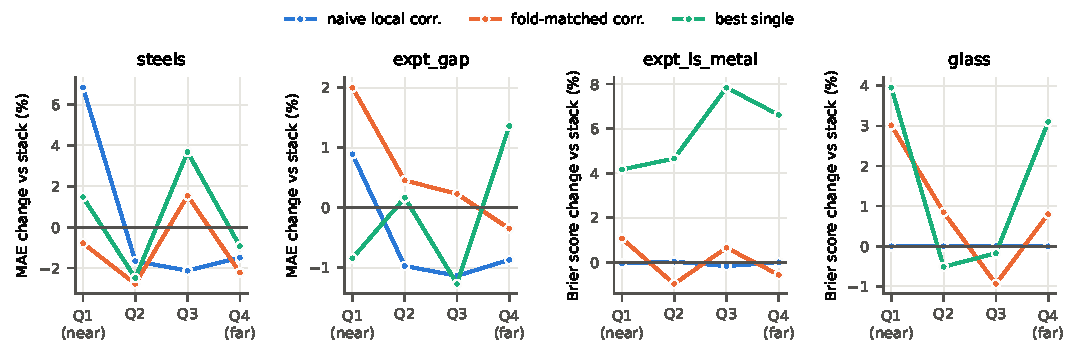
\includegraphics[width=\textwidth]{figures/fig_support.pdf}
\caption{Error change relative to the uncorrected stack, by support quartile (distance from the test composition to its nearest training composition; bin edges are the training rows' leave-one-out quartiles in each fold). Regression: MAE; classification: Brier score. Negative is better.}
\label{fig:support}
\end{figure}

\begin{figure}[t]
\centering
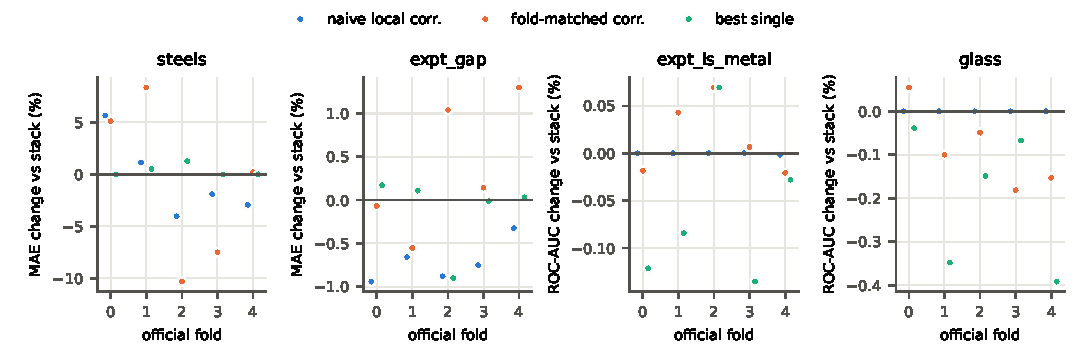
\includegraphics[width=\textwidth]{figures/fig_perfold.pdf}
\caption{Per-fold change of the test metric relative to the uncorrected stack for the naive and fold-matched corrections and the best single expert (selected by inner CV). For classification a positive change in ROC-AUC is better.}
\label{fig:perfold}
\end{figure}

\subsection{Ablations and controls}
Restricting the neighbour search to one composition space gave essentially the same gain on expt\_gap (Magpie \GapStackLocalMagpieVsStackRel\%, element fractions \GapStackLocalFracVsStackRel\%), whereas on steels only the element-fraction space was selected in practice and the Magpie-only variant was slightly worse than the stack (\SteelsStackLocalMagpieVsStackRel\%, 0/5 folds better).
Applying the correction to the best single expert instead of the stack (``correction without stacking'') improved expt\_gap by \GapSingleLocalVsBestSingleRel\% relative to that expert ($p_\mathrm{boot}=\GapSingleLocalVsBestSingleP$, 5/5 folds), so on this task the gain does not depend on stacking.
The label-permutation control did not behave as a clean null: with labels permuted within inner folds the selection still switched a correction on in every fold of every task (Table~\ref{tab:selections}), because shrinking predictions toward a neighbourhood mean lowers the training loss against permuted labels too.
We pre-registered this control as diagnostic only, and it shows that a non-zero selected strength is not by itself evidence of local structure.

\begin{table}[t]
\centering
\caption{Number of official folds (of 5) in which the inner-CV selection switched each correction on, and the same for the label-permutation control.}
\label{tab:selections}
\begin{adjustbox}{max width=\textwidth}
\begin{tabular}{lcccc}
\toprule
Task & naive corr. on & fold-matched corr. on & perm.\ control on (naive) & perm.\ control on (f.-m.) \\
\midrule
steels & 5/5 & 5/5 & 5/5 & 5/5 \\
expt\_gap & 5/5 & 5/5 & 5/5 & 5/5 \\
expt\_is\_metal & 1/5 & 5/5 & 5/5 & 5/5 \\
glass & 0/5 & 5/5 & 5/5 & 5/5 \\
\bottomrule
\end{tabular}

\end{adjustbox}
\end{table}

\subsection{Comparison with the Matbench leaderboard}
Table~\ref{tab:board} places the pre-registered primary arm on the leaderboard snapshot of 18 October 2026.
For the classification tasks we compare balanced accuracy at the inner-CV threshold with the board's balanced-accuracy column, because the board's ``ROC-AUC'' values of the label-based entries equal their balanced accuracy.
The method would rank \SteelsRank{} of \SteelsNEntries{} on steels (behind TPOT-Mat and AutoML-Mat, ahead of MODNet v0.1.12), \GapRank{} of \GapNEntries{} on expt\_gap (behind Darwin, ahead of the CrabNet and MODNet entries), \MetalRank{} of \MetalNEntries{} on expt\_is\_metal and \GlassRank{} of \GlassNEntries{} on glass.
It does not beat the best entry on any task.
On expt\_gap and glass the gaps to the leaders are large (\GapStackLocal{} vs.\ 0.2865~eV; balanced accuracy \GlassStackLocalBA{} vs.\ 0.9603), and on expt\_is\_metal it is 0.023 in balanced accuracy.
Our probability ROC-AUCs (\MetalAUCprob{} on expt\_is\_metal, \GlassAUCprob{} on glass) are not comparable with the label-based board values and are not ranked.

\begin{table}[t]
\centering
\caption{Primary arm versus the Matbench v0.1 leaderboard (snapshot 18 October 2026). Classification: balanced accuracy at the threshold chosen inside each training fold, compared with the board's balanced-accuracy column. Rank counts our entry among the board entries.}
\label{tab:board}
\begin{adjustbox}{max width=\textwidth}
\begin{tabular}{llccc}
\toprule
Task & Metric & Ours: stack + naive corr. & Best board entry & Rank \\
\midrule
steels & MAE & 82.80 $\pm$ 11.65 & TPOT-Mat: 79.95 $\pm$ 13.59 & 3 of 12 \\
expt\_gap & MAE & 0.3240 $\pm$ 0.0140 & Darwin: 0.2865 $\pm$ 0.0083 & 2 of 13 \\
expt\_is\_metal & balanced acc. & 0.9370 $\pm$ 0.0063 & Darwin: 0.9598 & 2 of 8 \\
glass & balanced acc. & 0.8841 $\pm$ 0.0184 & MODNet (v0.1.12): 0.9603 & 2 of 8 \\
\bottomrule
\end{tabular}

\end{adjustbox}
\end{table}

\subsection{Calibration and compute}
Stacking improved the Brier score and the expected calibration error over the best single expert on both classification tasks, and the corrections left them essentially unchanged (Table~\ref{tab:calib}).
On 24 CPU cores (5 parallel workers of 4 threads) one official fold took a median of about \SteelsScratchMin, \GapScratchMin, \MetalScratchMin{} and \GlassScratchMin{} minutes for steels, expt\_gap, expt\_is\_metal and glass when every expert was computed from scratch (the glass figure includes a system-standby pause); the pair-excluded refits of the fold-matched arm account for \SteelsPairShare\%, \GapPairShare\% and \MetalPairShare\% of the expert-fitting time on the first three tasks (\GlassPairShare\% on glass, inflated by the same pause).

\begin{table}[t]
\centering
\caption{Calibration on the classification tasks (means over folds) and balanced accuracy at the inner-CV threshold.}
\label{tab:calib}
\begin{adjustbox}{max width=\textwidth}
\begin{tabular}{llcccc}
\toprule
Task & Arm & Brier & log loss & ECE & bal.\ acc. \\
\midrule
expt\_is\_metal & Best single & 0.0498 & 0.2007 & 0.0369 & 0.9378 \\
expt\_is\_metal & Stack & 0.0469 & 0.1662 & 0.0201 & 0.9374 \\
expt\_is\_metal & Stack + naive corr. & 0.0468 & 0.1662 & 0.0192 & 0.9370 \\
expt\_is\_metal & Stack + fold-matched corr. & 0.0469 & 0.1660 & 0.0211 & 0.9366 \\
glass & Best single & 0.0747 & 0.2451 & 0.0220 & 0.8827 \\
glass & Stack & 0.0735 & 0.2398 & 0.0211 & 0.8841 \\
glass & Stack + naive corr. & 0.0735 & 0.2398 & 0.0211 & 0.8841 \\
glass & Stack + fold-matched corr. & 0.0740 & 0.2411 & 0.0232 & 0.8835 \\
\bottomrule
\end{tabular}

\end{adjustbox}
\end{table}

\begin{table}[t]
\centering
\caption{Mean simplex-stack weight per expert (over folds; ``--'' where the expert was not in the selected configuration of every fold).}
\label{tab:weights}
\begin{adjustbox}{max width=\textwidth}
\begin{tabular}{lcccc}
\toprule
Expert & steels & expt\_gap & expt\_is\_metal & glass \\
\midrule
et\_all & 0.94 & 0.86 & 0.41 & 0.57 \\
krr\_frac & 0.00 & 0.00 & -- & -- \\
krr\_magpie & 0.06 & 0.00 & -- & -- \\
lgbm\_all & 0.00 & 0.14 & 0.48 & 0.27 \\
lgbm\_l1\_all & -- & -- & -- & -- \\
mlp\_all & 0.00 & 0.00 & 0.05 & 0.00 \\
rf\_all & 0.00 & 0.00 & 0.03 & 0.10 \\
svc\_frac & -- & -- & 0.01 & 0.06 \\
svc\_magpie & -- & -- & 0.02 & 0.00 \\
\bottomrule
\end{tabular}

\end{adjustbox}
\end{table}

\section{Discussion}
\label{sec:discussion}

\paragraph{What the two pre-registered runs show}
The first run tested the transfer of the novelty-damped local OOF residual correction from our chemistry study.
It transferred only weakly: a consistent 0.7\% MAE gain on the experimental band gap, nothing measurable on steels, and nothing on the classification tasks, where the inner selection switched it off.
The second run strengthened the substrate instead. It added a disclosed DFT transfer block, a hurdle treatment of the zero-inflated band gap, more descriptors and more experts, and it gated the correction by a nested check.
That gate then kept the correction in none of the 20 folds.
The pipeline that emerges is therefore a well-regularised cross-fitted stack of standard composition experts. Its strength comes from \emph{what the experts see} (DFT descriptors) and \emph{what loss structure they model} (the point mass at $E_g=0$), not from a local residual stage.

\paragraph{The experimental band gap}
On expt\_gap the final pipeline's MAE differs from the board leader's by \AtwoRelGap\% (\AtwoFinalGap{} versus \AtwoLeaderGap~eV), and the margin is clear on a paired test.
Two caveats apply.
First, the gain relies on transfer from DFT calculations, which the leaders of this task do not use in the same form. We disclose it as transfer learning, use only the offline Materials Project data shipped with \texttt{matminer}, and use no experimental labels from outside the task.
Second, 27\% of the expt\_gap compositions have no DFT match, and for them the pipeline falls back on composition descriptors.
The hurdle construction is simple and general. A model that must predict exactly zero for half of the targets is poorly served by a single L1 or L2 regressor. Separating ``is the gap non-zero?'' from ``how large is it?'' removed a substantial part of that error in the design phase (MAE about 0.30 to 0.25 on fold~0's training rows).

\paragraph{The tasks where we do not lead}
On expt\_is\_metal and steels the pipeline is statistically on par with the leaders (Darwin and TPOT-Mat), and on glass it is clearly behind MODNet v0.1.12.
MODNet's glass submission reaches a probability ROC-AUC of \AtwoLeaderAUCGlass, against our \AtwoAUCGlass{}. We could not close this gap with the descriptors developed for glass formation or with any CPU-feasible expert we tried. A MODNet expert itself exceeded our CPU budget.
We did not audit the leaders' protocols. For example, we cannot tell from the public records whether all tuning was confined to the training folds. Our comparison is therefore against the reported numbers and predictions, not a claim about the methods.

\paragraph{Classification metrics on the leaderboard}
The leaders of both classification tasks are scored by balanced accuracy, whatever the column name says. Darwin recorded hard labels. MODNet recorded probabilities, but the \texttt{matbench} version that produced the board entry thresholded them at 0.5 for every metric.
A submission with probabilities scored by the current package would receive a true ROC-AUC (\AtwoAUCMetal{} for our expt\_is\_metal pipeline). That number is not comparable to the label-based entries.
We recommend that future submissions and leaderboards report balanced accuracy and probability ROC-AUC as separate columns.

\paragraph{Limitations}
\begin{itemize}
\item \textbf{Scope.} The study covers four composition tasks and CPU-feasible experts only. Five folds give little power per task, except where effects are large.
\item \textbf{Two looks at the test folds.} Amendment~2 was written after the Amendment-1 test results had been seen. Although every Amendment-2 choice was made on training rows only and the test folds were scored once under it, the decision to strengthen the pipeline, and the direction it took, were motivated by the first run's standing on the board. Both runs are reported in full.
\item \textbf{Candidate configurations from fold 0.} The candidate configurations, feature blocks and expert pool were developed on fold~0's training rows. Those rows contain the test rows of folds 1--4, so for those folds the \emph{space} of designs, though never their fitted parameters, was informed by data that later served as test data.
\item \textbf{Optimistic tuning OOF.} The Optuna-tuned expert's OOF predictions are mildly optimistic, because tuning and stacking share inner splits. This can affect only the stack weights.
\item \textbf{Dropped experts.} CrabNet- and MODNet-based experts were implemented but dropped for CPU cost, so the expert pool is not exhaustive.
\end{itemize}

\section{Conclusions}
\label{sec:conclusions}
We evaluated cross-fitted stacking of composition experts on the four Matbench v0.1 composition tasks under two pre-registered, fully nested protocols.

\textbf{First run.} A novelty-damped local OOF residual correction transferred only weakly from chemistry to materials.

\textbf{Second run.} The strengthened, still fully nested pipeline used DFT transfer descriptors and a hurdle model for the zero-inflated band gap. It:
\begin{itemize}
\item lowers the experimental band-gap MAE to \AtwoFinalGap~eV, below the current leader (\AtwoLeaderGap~eV);
\item is on par with the leaders on expt\_is\_metal and steels;
\item remains behind on glass.
\end{itemize}

We report all runs, folds and comparisons. Predictions and code are provided so that the numbers can be checked.


\section*{Data and code availability}
All code, the frozen analysis plan (\texttt{ANALYSIS\_PLAN.md}), SHA-256 freeze hashes, per-fold predictions of every arm, per-fold metrics and the unsubmitted Matbench result files are in the repository \url{https://github.com/bhaskargurram-ai/matbench-composition-stack}, which will be made public on submission. The data are the public Matbench v0.1 tasks.

\section*{Affiliation}
The author is an independent researcher with no institutional affiliation.

\section*{CRediT authorship contribution statement}
\textbf{Bhaskar Gurram:} Conceptualization, Methodology, Software, Formal analysis, Investigation, Writing -- original draft, Writing -- review \& editing.

\section*{Declaration of competing interest}
The author declares no competing financial interests or personal relationships that could have appeared to influence the work reported in this paper.

\section*{Declaration of generative AI and AI-assisted technologies in the writing process}
During the preparation of this work the author used Claude (Anthropic), running the ResearchStudio idea-generation skills, to assist with literature search, prior-art checking, code development and drafting of the manuscript. All analysis code, results and text were reviewed by the author, who takes full responsibility for the content of the publication.

\section*{Funding}
This research did not receive any specific grant from funding agencies in the public, commercial, or not-for-profit sectors.

\bibliographystyle{elsarticle-harv}
\bibliography{references}

\end{document}
